%\documentclass{article}
%\usepackage{amssymb}
%\usepackage{graphicx}
%\usepackage{caption}
%\usepackage{subcaption}
%\usepackage{listings}
%\usepackage{float} %figure inside minipage
%\graphicspath{ {./images/} }
%\usepackage[export]{adjustbox}
%\usepackage{apacite}
%
%\begin{document}

\chapter{Performance Analysis of Covid-19 PDE models with Discontinuities}
\label{chapter:pde}
\section{Introduction}
\label{subsection:pde_intro}
In this chapter, we present an investigation of the numerical solution of Covid-19 partial differential equation (PDE) models with discontinuities. Using a one dimensional (1D) PDE problem typically encountered in epidemiological studies (see, e.g., \cite{MR4126357}), we investigate the impacts on the accuracy and efficiency of the solution computed by an error-controlled solver when time-dependent and space-dependent discontinuities are introduced into the model.

As stated in the previous chapter, it is vital that numerical errors associated with the solutions computed by the solvers are negligible compared to the modeling errors associated with the mathematical and theoretical definition of the problem.

However, even more so than was the case for the Covid-19 ODE models, it is often the case that researchers will use PDE solvers that do not have error control. In Section $\ref{subsection:pde_software}$ we introduce BACOLIKR \cite{bacolikr} and explain its importance for the error-controlled numerical solution of PDEs. To our knowledge, BACOLIKR is also the only error-control PDE solver capable of event detection, which as shown in the previous chapter, becomes vital for the efficient computation of accurate solutions to state-dependent discontinuity problems.

In Section $\ref{subsection:pde_thrashing}$, we discuss thrashing in the presence of discontinuities for the PDE case and outline the impacts this has on the efficiency of error-controlled solvers. In Section $\ref{subsection:pde_software}$, we provide a description of BACOLIKR and, in Section $\ref{subsection:pde_problem_def}$, we give a description of the epidemiological model used in this chapter.

We provide a treatment of the time-dependent discontinuity PDE problem with and without discontinuity handling in Section $\ref{subsection:pde_time_intro}$ and a treatment of the state-dependent discontinuity PDE problem with and without event detection in Section $\ref{subsection:pde_state_intro}$.

\subsection{Thrashing in PDE models}
\label{subsection:pde_thrashing}
As was the case with ODE solvers, PDE solvers are also based on mathematical theories that assume that the solution and some of its higher derivatives are continuous. However, for the case of discontinuous problems, it has been observed that $\emph{error-control}$ solvers can accurately integrate through discontinuities. They do so at the cost of efficiency by repeatedly reducing the time step-size until the error of the step that takes the solver past the discontinuity satisfies the user-provided tolerance. This repeated reduction in the step-size implies that the solver must make a large number of function evaluations (i.e., evaluations of the right hand side of the PDE system) in a process called `thrashing'. This phenomenon was discussed for the ODE cased in Section $\ref{subsection:effect_of_discontinuity}$.

Thus, when a PDE solver integrates through a discontinuity, it repeatedly reduces the step-size at that discontinuity until the step-size is small enough to integrate through it. This leads to a spike in the number of function evaluations in the time interval near the discontinuity. Figure $\ref{fig:thrashing_pde}$ shows such a phenomenon. A PDE problem with a discontinuity at $t=30$ is solved and we plot the cumulative number of function evaluations at each time step. We see a spike in the number of function evaluations at $t=30$.
\begin{figure}[H]
\centering
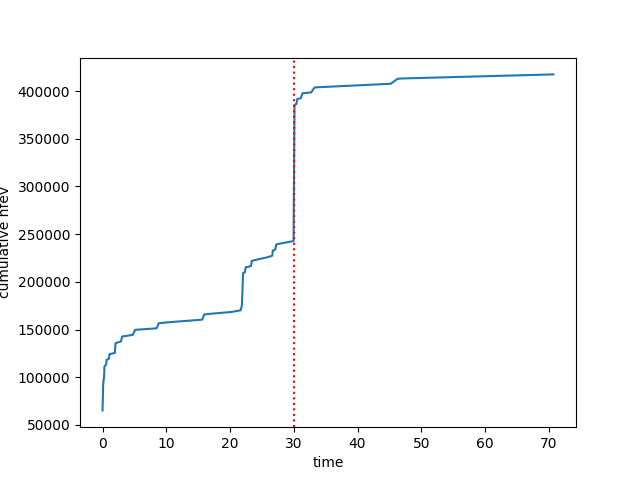
\includegraphics[width=0.7\linewidth]{./figures/pde_thrashing}
\caption{Thrashing in the PDE context}
\label{fig:thrashing_pde}
\end{figure}

In this chapter, we will show that a PDE solver with error-control, such as BACOLIKR, can integrate through a time-dependent discontinuity but that discontinuity handling leads to a more efficient solution.
(See Section $\ref{subsection:pde_time_intro}$). We will also show that state-dependent discontinuity problems cannot be accurately solved without event detection (See Section $\ref{subsection:pde_state_intro}$).

\subsection{BACOLIKR, an error-control PDE solver with event detection capability}
\label{subsection:pde_software}
BACOLIKR \cite{bacolikr} is a member of the BACOL family of 1D PDE solvers. Its underlying principle is that it solves PDE problems  by employing a discretisation of the spatial domain using B-spline collocation; the B-spline collocation method is based on a spatial mesh of points that partitions the spatial domain. The collocation method is applied on the spatial domain to approximate the PDE system with a larger time-dependent ODE system. This ODE system together with the boundary conditions, represents a time-dependent system of Differential-Algebraic Equations (DAEs) which are solved using the DAE solver, DASKR (a DAE solver with root-finding capabilities) \cites{MR1298625}{MR1618796}. DASKR provides adaptive time-stepping and adaptive method order selection to control the error of the time integration component of the computation. BACOLIKR also provides control over the spatial error through adaptive refinement of the spatial mesh. It uses interpolation schemes to obtain low-cost spatial error estimates for the numerical solution that it computes. Based on the spatial error estimate, the spatial error can be controlled by increasing or decreasing the number and the locations of spatial mesh points. See \cite{bacolikr} for further details.

BACOLIKR tries to satisfy a user-provided tolerance in the most efficient way possible using an adaptive spatial mesh and adaptive time-stepping and method order selection. By using the root-finding DAE solver DASKR, BACOLIKR can also perform event detection and thus can be used to handle discontinuities in a manner that is similar to what we saw in the ODE case in the previous chapter. We wish to emphasize these two important qualities of BACOLIKR, i.e., the error control and the event detection capability, as they provide a level of accuracy and efficiency that other PDE solvers, especially rudimentary ones, very rarely grant, for these types of problems.

\subsection{Problem Definition}
\label{subsection:pde_problem_def}
In this chapter, the PDE model we will investigate is an SEIR model that uses a spatial variable, $x$, and a time variable, $t$. Similar PDE models have been used in other applications (see \cite{MR3406651}). Here we will represent the spread in geographical location using the spatial variable.

In this chapter, a PDE problem is described using a system of PDEs of the form:
\begin{equation}
u_t(x, t) = f(x, t, u(x,t), u_x(x,t), u_{xx}(x,t)),
\end{equation} 
over a spatial domain ${a \leq x \leq b}$ and a temporal domain [${t_0}$, $t_{final}$]. 

It requires a set of initial conditions of the form:
\begin{equation}
u(x, t) = u_0(x),
\end{equation}
for $x$ in the spatial domain, ${a \leq x \leq b}$.

It also requires boundary conditions of the form:
\begin{equation}
b_L(t, u(a,t), u_x(a,t)) = 0, \quad b_R(t, u(b,t), u_x(b,t)) = 0,
\end{equation} 
for time, $t \geq t_0$.

We define an SEIR model based on the one developed in \cite{pdeModel} and given below. The model is obtained by introducing diffusion terms into the ODEs that we saw in the previous chapter.

The system of PDEs is:
\begin{equation}
S(x, t)_t = D_S(x)S(x, t)_{xx} + \mu N - \mu S(x, t) - \frac{\beta}{N}S(x, t)I(x, t),
\end{equation}
\begin{equation}
E(x, t)_t = D_E(x)E(x, t)_{xx} + \frac{\beta}{N}S(x, t)I(x, t) - \alpha E(x, t) - \mu E(x, t),
\end{equation}

\begin{equation}
I(x, t)_t = D_I(x)I(x, t)_{xx} + \alpha E(x, t) - \gamma I(x, t) - \mu I(x, t),
\end{equation}

\begin{equation}
R(x, t)_t = D_R(x)R(x, t)_{xx} + \gamma I(x, t) - \mu R(x, t).
\end{equation} 

The spatial domain is $-5 \leq x \leq 5$ and the temporal domain is $0 \leq t \leq 70$ for the time-dependent discontinuity problem and $0 \leq t \leq 200$ for the space-dependent discontinuity problem.

The parameters for the above SEIR model are as follows: $\mu$, the birth/death rate, is set to $\frac{0.01}{365}$, $\gamma$, the recovery rate is 0.06, $\alpha$, the incubation rate is 0.125, and we will vary the transmission rate, $\beta$, between 0.035 and 0.9 based on whether measures, such as social distancing, etc., are implemented in the model. The population size, N, is $3.7 \times 10^{7}$.

The model also uses diffusion coefficients,  $D_S(x)$, $D_E(x)$, $D_I(x)$ and $D_R(x)$, to model the spread of the virus over the spatial domain. These are defined as follows:
\begin{equation}
D_S(x) = D_E(x) = D_R(x) = (maxD_s - minD_s)e^{-10(\sqrt{x^{2}} - 1)^2)} + minD_s,
\end{equation} 
\begin{equation}
D_I(x) = D_E(x)/10,
\end{equation}
where the diffusivity parameters $maxD_s$ and $minD_s$ are 0.8 and 0.01, respectively. See Figure $\ref{fig:pde_D_s}$ for a plot of $D_s(x)$. This represents the case, for example, when the population density is quite high and where there are clusters of unvaccinated people in certain regions, and thus the disease can diffuse through the population in those regions more quickly. These regions are centered at $x= \pm 1$ in our model.

\begin{figure}[H]
\centering
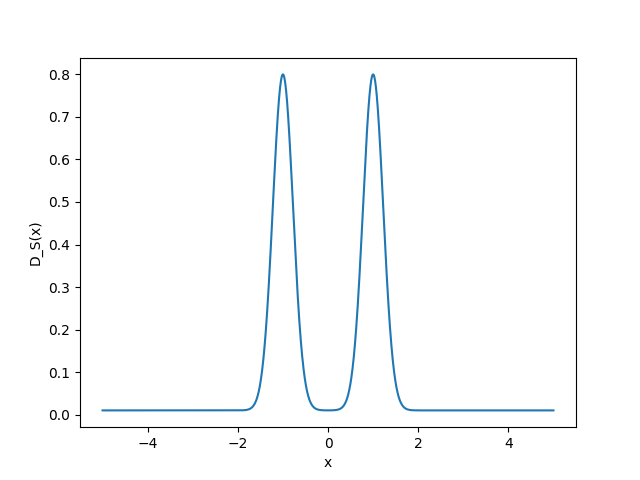
\includegraphics[width=0.7\linewidth]{./figures/pde_D_s}
\caption{Plot of the diffusion coefficient $D_S(x)$}
\label{fig:pde_D_s}
\end{figure}

The set of initial conditions are defined over the spatial domain as follows:
\begin{equation}
S(x, 0) = N - I(x, 0),
\end{equation}
\begin{equation}
I(x, 0) = 100e^{-x^2},
\end{equation}
\begin{equation}
E(x, 0) = R(x, 0) = 0.
\end{equation}
These initial conditions represent the case where there is a relatively small group of infected people at the location corresponding to $x=0$. (See Figure $\ref{fig:pde_I_0}$).

\begin{figure}[H]
\centering
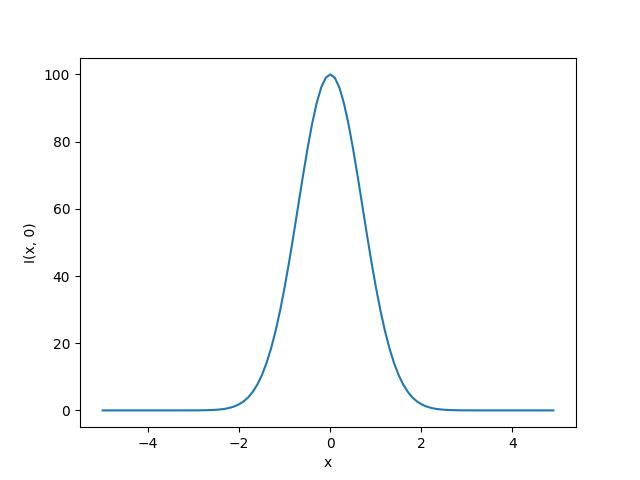
\includegraphics[width=0.7\linewidth]{./figures/pde_I_0}
\caption{Plot of the initial condition I(x, 0)}
\label{fig:pde_I_0}
\end{figure}

The boundary conditions are Neumann boundary conditions whereby the spatial derivative for each solution component at each boundary is required to be zero.

The above gives us a complete PDE problem definition. To this problem we will add discontinuities as follows. 
In the time-dependent discontinuity case (Section $\ref{subsection:pde_time_intro}$), we will integrate the model with $\beta$ at a value of 0.9 from $t=0$ to $t=30$; we will then change the value of $\beta$ to 0.035 and integrate until $t=70$. This change in the parameter introduces a discontinuity into the right hand side of the PDE system. This simulates a scenario where 30 days into a pandemic, measures are introduced to slow the spread of the pathogen.

In the state-dependent discontinuity problem (Section $\ref{subsection:pde_state_intro}$), we start the integration with the value of $\beta$ equal to 0.9 and use this value as we integrate forward in time until the spatial integral of $E(x, t)$, i.e, the total number of exposed people across the spatial domain at time, t, is 30000. When that integral value reaches 30000, we change the value of $\beta$ to 0.035 and keep it at this value until the integral value of $E(x, t)$ over the spatial domain decreases to 10000. We then switch the model and continue with a value $\beta$ of 0.9. We repeat this process until $t=200$. This process simulates a series of introducing and relaxing measures, such as social distancing, based on the total number of exposed individuals across the whole region.

\section{Time Dependent Discontinuity Model}
\label{subsection:pde_time_intro}
In this section, we investigate the numerical solution computed by BACOLIKR for the Covid-19 PDE model with a time-dependent discontinuity. The time-dependent discontinuity is introduced by changing the value of the SEIR modeling parameter, $\beta$ from 0.9 to 0.035 at $t=30$.

We note that this section demonstrates that the PDE time-dependent discontinuity PDE problem is similar to the ODE time-dependent discontinuity problem. We will show that reasonably accurate solutions can be computed without the use of discontinuity handling but that the use of discontinuity handling through the use of a cold start dramatically improves the efficiency of the computation.

For the following sections, we will plot $E(x, t)$ at $x=0$ to show both that the problem initially has an exponentially growing solution component and the rapid change of that component to exponential decay when the parameter $\beta$ is reduced.

\subsection{Simple treatment of the time-dependent discontinuity PDE model}
\label{subsubsection:pde_time_naive}
The simple treatment for time-dependent discontinuities is to use if-statements in the right-hand side function based on the value of the time argument, $t$, and to use the default tolerance.

For our model, we start with a value of $\beta$ at 0.9 and from $t=30$ onwards, the value for $\beta$ is reduced to 0.035. The pseudo-code for this approach is as follows:

\begin{minipage}{\linewidth}
\begin{lstlisting}[language=Python]
function model_with_if(t, x, u, ux, uxx)
	// ...
	beta = 0.9
	if t >= 30:
		beta = 0.035
	// ...
	return (dSdt, dEdt, dIdt, dRdt)

\end{lstlisting}
\end{minipage}

This change in the $\beta$ parameter introduces a discontinuity in the model, which leads to thrashing as discussed in Section $\ref{subsection:pde_thrashing}$. However as we have shown in Section $\ref{section:time_problem}$ for the ODE case, error-control PDE solvers can also reduce the time step-size to integrate through a time-dependent discontinuity with reasonable accuracy. (See Figure $\ref{fig:pde_time_disc_naive}$.)

\begin{figure}[H]
\centering
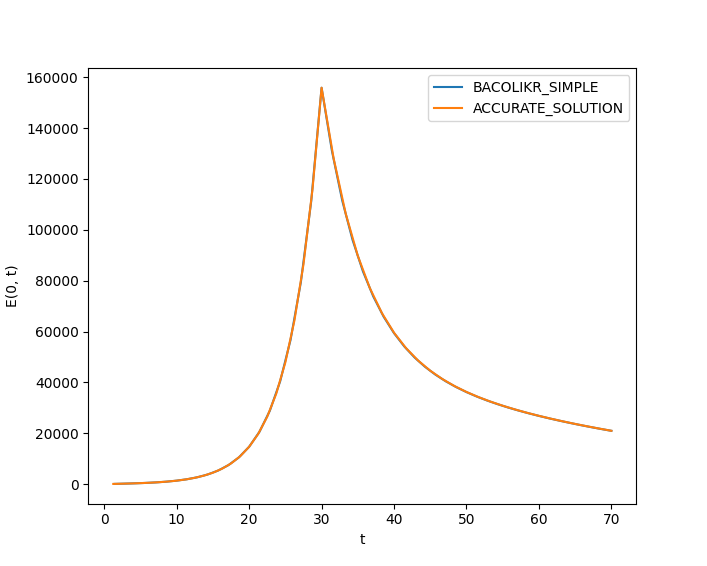
\includegraphics[width=0.7\linewidth]{./figures/pde_time_disc_naive}
\caption{Simple treatment of the time dependent discontinuity Covid-19 Model (with a tolerance of $10^{-6}$)}
\label{fig:pde_time_disc_naive}
\end{figure}

From Figure $\ref{fig:pde_time_disc_naive}$, we can see that the computed solution is in good argument with a high accuracy solution obtained from a computation with discontinuity handling at a very sharp tolerance. Though the solution without discontinuity handling is accurate, in the next section, we will show how a cold start can give the same level of accuracy while using fewer function evaluations.

\subsection{Discontinuity handling for the time-dependent discontinuity PDE model}
\label{subsubsection:pde_time_disc_hand}
In this section, we discuss the use of discontinuity handling through the introduction of cold starts. Though the error-controlled solver, BACOLIKR, was able to get accurate solutions without discontinuity handling, we will show that the use of cold starts allows it to be more efficient.

Recall that a solver is said to perform a cold start when it restarts by clearing all its data structures, reducing the time step-size to the small initial step-size, and reducing its time stepping method to first order (in the case where a variable order DAE solver is employed). This way the solver does not allow any effects from previous steps to influence the next step. Modern PDE solvers like BACOLIKR have flags that a user can set to force it to perform a cold start. We will use such a flag to set a cold start when one is needed.

The idea for performing time-dependent discontinuity handling is to use BACOLIKR to solve up to the discontinuity, cold start at the discontinuity, and then solve to $t_{final}$. In our case, we solve the problem with one call from $t=0$ to $t=30$ using 0.9 for the value of the $\beta$ parameter. We then restart with a cold start and integrate from $t=30$ to the end of the time interval with another call to the solver using $\beta$ equal to 0.035. The pseudo-code for this approach is as follows

\begin{minipage}{\linewidth}
\begin{lstlisting}[language=Python]
function model_before(t, x, u, ux, uxx):
	// ...
	beta = 0.9
	// ...
function model_after(t, x, u, ux, uxx):
	// ...
	beta = 0.035
	// ...

solution = pde_solver.init(...)
tspan_before = [0, 30]
pde_solver(solution, model_before, tspan_before)

solution.cold_start_flag = True

tspan_after = [30, 70]
pde_solver(solution, model_after, tspan_after)

\end{lstlisting}
\end{minipage}

\begin{figure}[H]
\centering
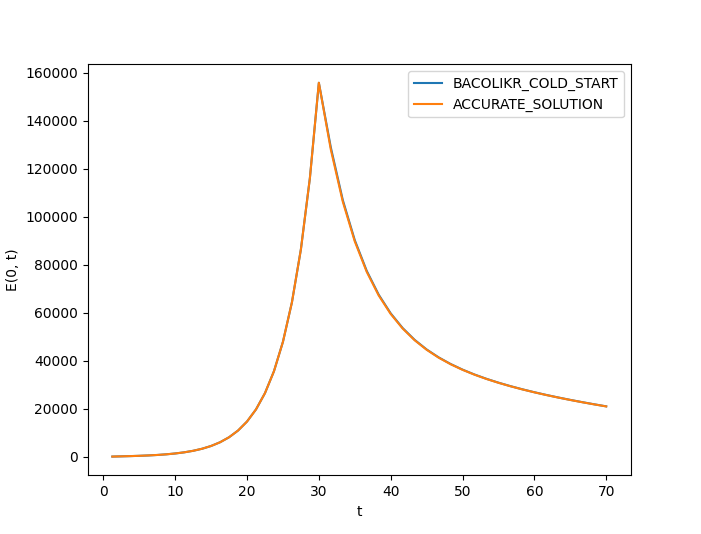
\includegraphics[width=0.7\linewidth]{./figures/pde_time_disc_disc_hand}
\caption{Discontinuity handling for time discontinuity problem (with a tolerance of $10^{-6}$)}
\label{fig:pde_time_disc_disc_hand}
\end{figure}

As expected, Figure $\ref{fig:pde_time_disc_disc_hand}$ shows that BACOLIKR with the cold start is able to provide a solution with the same accuracy as it did without the cold start. We now note however that the use of a cold start allows the solver to make 359755 function evaluations whereas when the solver is used without a cold start, it required 417505 function evaluations. We were thus able to make around 50000 fewer function evaluations when discontinuity handling is employed which amounts to around a $14\%$ gain in efficiency.

\subsection{PDE time-dependent discontinuity problem tolerance study}
\label{subsubsection:pde_time_tol}

As was the case with the Covid-19 ODE model, a researcher might want to coarsen the tolerance if they need to run the solver in a loop or within an optimization algorithm (see Appendix $\ref{section:ebola_paper}$) in order to improve the speed of the computation. We therefore now perform a tolerance study on this time-dependent discontinuity problem to see whether discontinuity handling allows us to use coarser tolerances as it did in the ODE case. We will also consider the use of sharper tolerances to show how the use of discontinuity handling significantly improves the efficiency.

Figures $\ref{fig:pde_time_disc_bacolikr_naive_tol}$ shows the solutions obtained without discontinuity handling at the different tolerances, while Figure $\ref{fig:pde_time_disc_bacolikr_disc_hand_tol}$ shows the solutions obtained with discontinuity handling at the different tolerances. We plot $E(x, t)$ at $x=0$ in both cases. 

\begin{figure}[H]
\centering
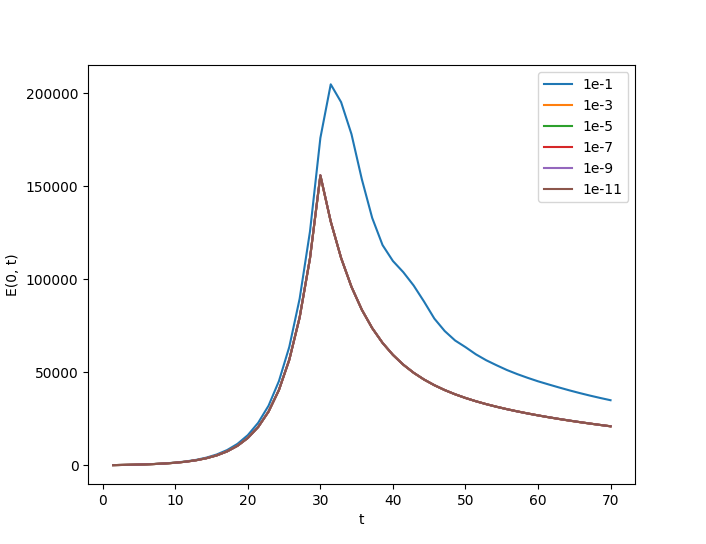
\includegraphics[width=0.7\linewidth]{./figures/pde_time_disc_bacolikr_naive_tol}
\caption{Time dependent discontinuity tolerance study with BACOLIKR without discontinuity handling.}
\label{fig:pde_time_disc_bacolikr_naive_tol}
\end{figure}

\begin{figure}[H]
\centering
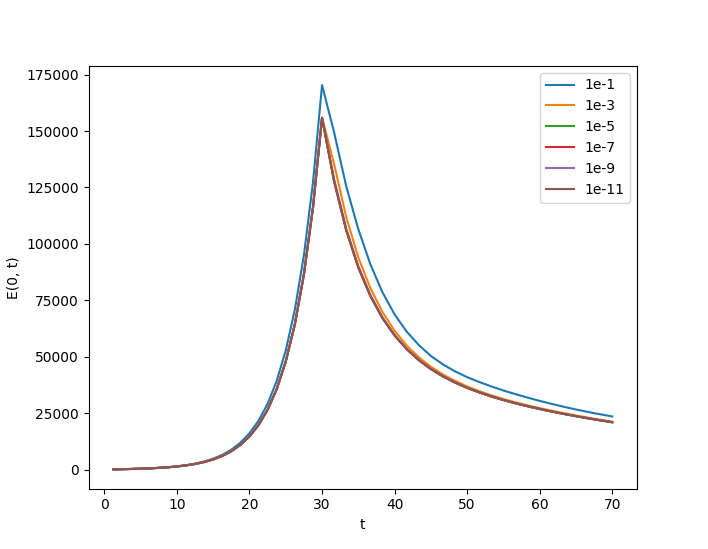
\includegraphics[width=0.7\linewidth]{./figures/pde_time_disc_bacolikr_disc_hand_tol}
\caption{Time dependent discontinuity tolerance study with BACOLIKR using discontinuity handling.}
\label{fig:pde_time_disc_bacolikr_disc_hand_tol}
\end{figure}

We note that both for the case with discontinuity handling and for the case without discontinuity handling, the solutions computed using a tolerance of $10^{-1}$ are inaccurate. We note that surprisingly, the discontinuity handling solution at a tolerance of $10^{-3}$ is more accurate without discontinuity handling than with. We explain this fact by noting that the step-size at a tolerance of $10^{-3}$ was much smaller than required in the case without discontinuity handling than in the case with discontinuity handling. Thus, although the solution is more accurate, the solver without discontinuity handling is inefficient as it could have satisfied this tolerance with a much larger step-size. This can be seen in Table $\ref{tab:pde_time_nfev}$ where we can see that the solver without discontinuity handling performs about 2500 more function evaluations than required. For all tolerances sharper than $10^{-3}$, the solutions are all reasonably accurate.

\begin{table}[h]
\caption {PDE time discontinuity tolerance study - number of function evaluations} 
\label{tab:pde_time_nfev}
\begin{center}
\begin{tabular}{ c c c } 
tolerance & BACOLIKR simple  & BACOLIKR disc hand \\ 
1e-1      &   40800         &   55400 \\
1e-3      &   79220         &   76750 \\
1e-5      &  206980         &  208870 \\
1e-7      &  733210         &  543850 \\
1e-9      & 1904080         & 1653830 \\
1e-11     & 7140875         & 4979555 \\
\end{tabular}
\end{center}
\end{table}

Table $\ref{tab:pde_time_nfev}$ shows the improvement in efficiency when discontinuity handling is employed. We note that the smaller number of function evaluations for the case without discontinuity handling at a tolerance of $10^{-1}$ is not relevant because the solutions at this tolerance are very inaccurate. At a tolerance of $10^{-5}$, the discontinuity handling does more function evaluation than without. We then note that for any of the sharper tolerances, the use of discontinuity handling leads to a gain in efficiency and that at very sharp tolerance such as $10^{-11}$, the solver does around 2 million fewer function evaluations with a cold start than without (around a $30\%$ gain in efficiency). 

\section{State Dependent Discontinuity Model}
\label{subsection:pde_state_intro}
In this section, we discuss the state-dependent discontinuity problem. Again, we note that state-dependent discontinuity problems are not as trivial as time-dependent discontinuity problems and that for these problems, we do not have a straightforward way to introduce a cold start since we do not know when the discontinuities will arise. We will also attempt a longer integration in this section as we will run the solver to $t=200$ to see for how long a period of time the solver can provide accurate solutions.

In state-dependent discontinuity problems, we use the value of one of the components of the solution to dictate how the model should behave. We compare one the solution component against a pre-determined threshold and if this threshold is crossed, we change the model. However, unlike, in the ODE case, in the PDE case, we have another dimension, the spatial dimension, to consider. Some of the ways to include the spatial dimension are listed below:
\begin{itemize}
\item Consider a spatial value, say $x=0$, and sample the solution component at this spatial point at the end of every time step. If the solution component value meets a certain threshold, we apply a different model, otherwise we continue with the same model

\item Compute some statistical measure of the solution component (e.g., min, max, average) across the spatial domain and use that value for the comparison with the threshold.

\item Integrate the solution component over the spatial domain and use that integral value for the comparison against the threshold.
\end{itemize}

In this chapter, we will use the third method. If the value of the integral of the solution component reaches a maximum threshold (30000), the value of the parameter $\beta$ is changed from 0.9 to 0.035 and when we cross a certain minimum threshold (10000), the value of the parameter $\beta$ is changed back to 0.9. This models the situation where a government looks at the total number of cases over all geographical locations to inform a decision regarding introducing/relaxing measures.

Again, we note that a discontinuity is introduced by the change in the parameter $\beta$.

For the following sections, we will plot the integral value of $E(x, t)$ over the spatial dimension. An accurate solution will thus have an integral oscillating cleanly between 10000 and 30000 as the model is changed.

\subsection{Simple treatment of the state-dependent discontinuity model}
\label{subsubsection:pde_state_naive}
Similar to the approach used for the ODE case in the previous chapter, a simple treatment of this problem involves using global variables which are toggled based on the integral value over the spatial domain to denote which model to use. The global variable selects which value of $\beta$ to use in the model function. When measures are implemented, the value of $\beta$ is 0.035; when measures are not implemented the value of $\beta$ is 0.9.

In this simple implementation, the user will have to specify the times at which the solver should stop and run an integration over the spatial domain to get a value to compare against the thresholds. This form of `manual' time-checking introduces another parameter, the `number of time intervals', that the user will have to fine-tune in order to obtain accurate results. We will show, in this section and the next section, why this parameter is very difficult to get right despite how crucial it is for the goal of obtaining accurate results. If the number of time intervals is too small, we will toggle the global variable too late as we will check the integral value after it had already crossed the threshold and if the number of time intervals is too large, we will check the integral value too often which will reduce the efficiency. 

The simple approach will be to divide the time domain into $num\_time\_intervals$ equal intervals. The solver will solve the model from the beginning of each time interval to the end of that time interval. At the end of each interval, the solver will estimate the integral of $E(x, t)$ using a compound trapezoidal rule \cite{heath2018scientific}. This integral value will be compared against the threshold and if measures are not implemented and the integral is greater than 30000, the maximum threshold, the global variable indicating that measures are implemented will be switched to true and the parameter $\beta$ will be set to 0.035. When measures implemented and the integral value is less than 10000, the minimum threshold, the global variable is switched to false indicating that $\beta$ is now at 0.9, corresponding to measures being relaxed. The pseudo-code for this approach is as shown:

\begin{minipage}{\linewidth}
\begin{lstlisting}[language=Python]
measures_implemented = False

function model(t, x, u, ux, uxx):
	// ...
	global measures_implemented
	if (measures_implemented):
		beta = 0.035
	else:
		beta = 0.9
	// ...

tstart = 0
tstop = 200
num_time_intervals = 400
time_step_size = (tstop - tstart) / num_time_intervals
solution = pde_solver.init(...)

t_current = tstart
t_next = t_current + time_step_size

while t_current < tstop:
	tspan = [t_current, t_next]
	pde_solver(solution, model, tspan)
	integral_value = integrate( spatial_interpolate(solution) )
	if (not measures_implemented):
		if (integral_value >= 30000): 
			measures_implemented = True
	else:
		if (integral_value <= 10000):
			measures_implemented = False
t_current = t_next
t_next = t_next + time_step_size
\end{lstlisting}
\end{minipage} 

Figure $\ref{fig:pde_state_disc_naive_400vs1000}$ shows the integral value of $E(x, t)$ over the spatial domain with 400 time intervals and with 1000 time intervals together with a high accuracy solution obtained via event detection using a sharp tolerance. We can see that neither of the solutions obtained using the simple approach are in agreement with the high accuracy solution. In the next section, we will explain why the simple implementation cannot obtain an accurate solution, and in the section after that, we will show how event detection provides a better way to solve this problem.

\begin{figure}[H]
\centering
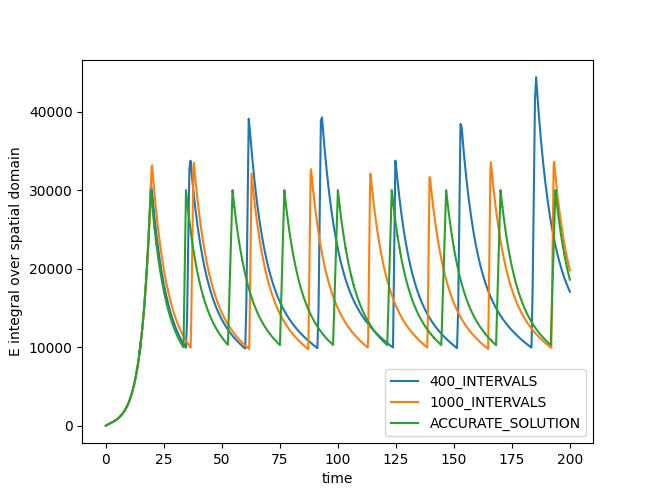
\includegraphics[width=0.7\linewidth]{./figures/pde_state_disc_naive_400vs1000}
\caption{Integral value of $E(x, t)$ from a simple treatment of the state-dependent discontinuity problem with a tolerance of $10^{-6}$ using 400 and 1000 time intervals, compared with a high accuracy solution}
\label{fig:pde_state_disc_naive_400vs1000}
\end{figure}

\subsection{Why the simple approach cannot give an accurate solution}
\label{subsubsection:pde_state_naive_always_inaccurate}
The simple method cannot solve the problem accurately because of the issue of choosing the correct number of time intervals. The check in which we compare the integral of $E(x, t)$ against the thresholds can only be performed at the end of a time interval. Thus we can detect that the thresholds are crossed only after they have been crossed rather than exactly at the point where a threshold is crossed.

One idea to address this issue would be to use an exceedingly large number of time intervals (e.g., 10000) so that we only take a small number of time steps with the wrong $\beta$ value. Figure $\ref{fig:pde_state_disc_naive_1000vs10000}$ shows how doing so produces a solution more in line with the high accuracy, event-detection solution. However, even this plot does not approach the accurate solution, especially at later times. 

\begin{figure}[H]
\centering
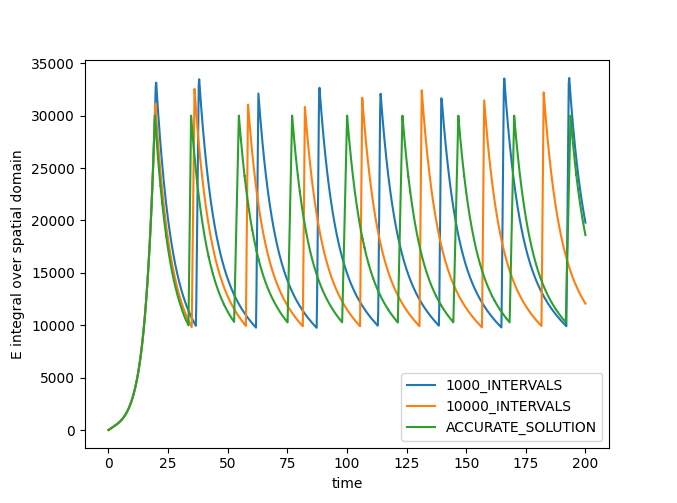
\includegraphics[width=0.7\linewidth]{./figures/pde_state_disc_naive_1000vs10000}
\caption{Integral value of $E(x, t)$ from a simple treatment of the state-dependent discontinuity problem with a tolerance of $10^{-6}$ using 1000 and 10000 time intervals, compared with a high accuracy solution}
\label{fig:pde_state_disc_naive_1000vs10000}
\end{figure}

We could use an even larger number of time intervals but using such a high number of time intervals will lead to a substantial loss in efficiency. A much better option is to use event detection. In the next section, we will show how event detection provides an intuitive, efficient and accurate way of solving such problems. It will allow us to correctly cold start when needed and thus have BACOLIKR integrate only on continuous sub-problems of the state-dependent discontinuity problem. It will also find the time at which the value of the integral of $E(x, t)$ crosses a threshold and will improve the efficiency of the computation as well.

\subsection{Event detection solution to the state-dependent discontinuity model}
\label{subsubsection:pde_state_event_detection}
In the previous section, we have explained the issue with using manual time-step checking to obtain an accurate solution. In this section, we will present event detection for the PDE case, explain how it leads to more accurate results and explain how it makes the minimum number of calls to the integration routine required to obtain an accurate solution.

As mentioned earlier, BACOLIKR is an error control PDE solver with an event detection capability. Event detection also works in the same way as it does in the ODE case. To use event detection, the user provides a root function to the PDE solver. The root function uses the solution available over the current time step to evaluate an event function. A root is detected when the returned value of the event function is 0. After each time step, the solver calls the root function providing it with the solution on the current time step together with the current spatial mesh. If the returned value from the root function changes sign between two consecutive steps, a root is present in the current step. The solver will then employ a root-finding algorithm within the time-step to find the time at which the root function is zero. The solver then returns, setting flags indicating that it has found a root and providing the solution at the root. 

To solve the state-dependent discontinuity problem, we define two pairs of root and model functions. One pair is used for the case when there are no measures in place. The model function will have the parameter $\beta$ set to a value of 0.9 and the root function that performs the integration of $E(x, t)$ over the spatial domain for the current time step will return the difference between the integral value and the maximum threshold (30000). The second pair will have a model function with $\beta$ set to a value of 0.035 and the root function will return the difference between the integral of $E(x, t)$ and the lower threshold value of 10000. The solver starts with the first pair of functions as initially measures are not implemented. It will return when the 30000 maximum threshold is met. At this point, the cold start flag is set and the solver is called to continue with the second pair of model-root functions. The solver will now return when the integral of the $E(x, t)$ equals 10000. When that happens, we perform a cold start and run the solver with the first model-root function pair. We repeat this process until the solver reaches $t=200$. The pseudo-code for this approach is as follows:

\begin{minipage}{\linewidth}
\begin{lstlisting}[language=Python]
function model_no_measures(t, x, u, ux, uxx):
	// ...
	beta = 0.9
	// ...
function root_max_value(t, solution):
	// ...
	integral_value = integrate( spatial_interpolate(solution) )
	return integral_value - 30000
function model_with_measures(t, x, u, ux, uxx):
	// ...
	beta = 0.035
	// ...
function root_min_value(t, solution):
	// ...
	integral_value = integrate( spatial_interpolate(solution) )
	return integral_value - 10000

tstart = 0
tstop = 200
t_current = tstart
measures_implemented = false

while t_current < tstop:
	tspan = [t_current, t_stop]
	if (measures_implemented):
		pde_solver(solution, model_with_measures, 
			tspan, root_min_value)
	else:
		pde_solver(solution, model_no_measures, 
			tspan, root_max_value)
	
	if (solution.root_flag == True):
		solution.cold_start_flag = True
		// switch model-root pair
		measures_implemented = not measures_implemented
	t_current = solution.t

\end{lstlisting}
\end{minipage}

Figure $\ref{fig:pde_state_disc_event_tol_6}$ shows the solution we obtain using a tolerance of $10^{-6}$ and using event detection to solve the state-dependent discontinuity problem. We can see that the solution correctly oscillates between 10000 and 30000 and that for the first few oscillations, it lines up with the highly accurate solution. We then see that although it oscillates correctly, at later times, it is not completely aligned with the high accuracy solution. 

\begin{figure}[H]
\centering
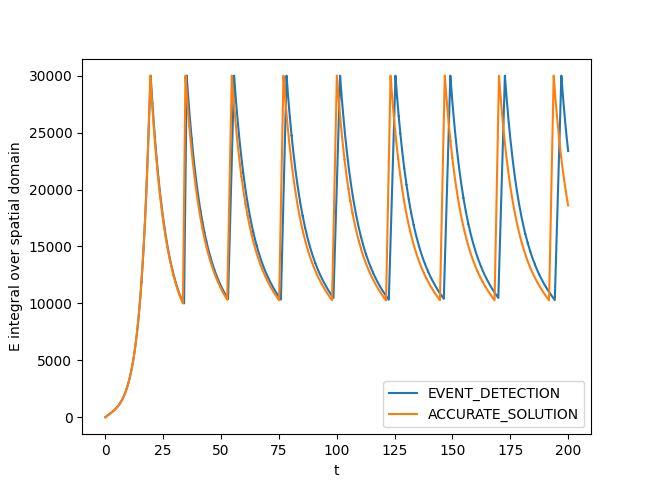
\includegraphics[width=0.7\linewidth]{./figures/pde_state_disc_event_tol_6}
\caption{Integral value plot of the event detection solution to state-dependent discontinuity problem with a tolerance of $10^{-6}$}
\label{fig:pde_state_disc_event_tol_6}
\end{figure}

We explain this misalignment by noting that the root-detection algorithm employed inside BACOLIKR detects a root based on the tolerance. It signals that it has detected a root when the root function value is within the tolerance. Thus if we sharpen the tolerance and run the same experiment, the solutions obtained using sharper tolerances will tend to align themselves more with the high accuracy solution.

Figure $\ref{fig:pde_state_disc_event_tol_9}$ shows the result of solving this problem at a tolerance of $10^{-9}$. At this higher tolerance, the root is detected when the root function returns with a value within a tolerance of $10^{-9}$. Thus the solver approaches the correct root times more accurately and the solutions are more aligned with the high accuracy solution, especially at the later times, compared to the solution at a tolerance of $10^{-6}$.


\begin{figure}[H]
\centering
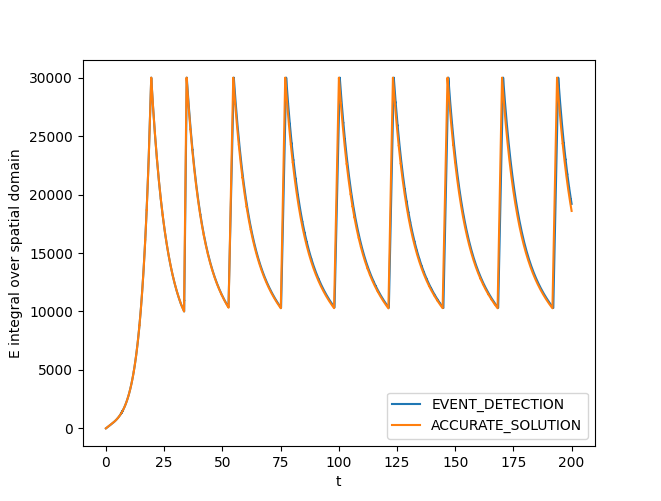
\includegraphics[width=0.7\linewidth]{./figures/pde_state_disc_event_tol_9}
\caption{Integral value plot of the event detection solution to state-dependent discontinuity problem with a tolerance of $10^{-9}$}
\label{fig:pde_state_disc_event_tol_9}
\end{figure}

We now note that both solutions with event detection, even the one computed using a tolerance of $10^{-6}$ are much more accurate than the simple solutions that were computed using manual selection of the time intervals. Table $\ref{tab:pde_state_nfev}$ shows the number of function evaluations. 

\begin{table}[h]
\caption {PDE state discontinuity model - number of function evaluations} 
\label{tab:pde_state_nfev}
\begin{center}
\begin{tabular}{ c c } 
method & nfev \\ 
simple implementation with 400 steps   & 1184880 \\
simple implementation with 1000 steps  & 1280080 \\
simple implementation with 10000 steps & 1272030 \\
event detection at $10^{-6}$ tol.     & 1937730 \\
event detection at $10^{-9}$ tol.     & 7915085 \\
\end{tabular}
\end{center}
\end{table}

Table $\ref{tab:pde_state_nfev}$ shows that event detection required more function evaluations than the solutions without event detection. However these non-event detection solution were very inaccurate and thus the associated function evaluation counts are not relevant. 

We also discuss the fact that that the number of function evaluations is not the only measure of efficiency in this case as we also need to consider the number of times the integration routine is called. We note that for the simple implementation, if we are using $n$ time intervals, then the integration routine is called $n$ times. For the event detection approach, the number of times the integration routine is called is the number of times the root function is called. With a tolerance of $10^{-6}$, the integration routine is called 2149 times and with a tolerance of $10^{-9}$, the integration routine is called 5059 times. We note that the integration routine is thus called less than 10000 times in both cases and that the simple implementation did not get accurate results even with 10000 calls to the integration routine.

We now note that even with event detection, we are faced with the problem of finding a good trade-off between efficiency and accuracy. Improving the accuracy comes at the price of efficiency. In the next section, we will perform a tolerance study to analyze this trade-off.

\subsection{State-dependent discontinuity problem tolerance study}
\label{subsubsection:pde_state_tol_study}
In this section, we perform a tolerance study on the different solutions to the state-dependent discontinuity problem. We use the simple implementation with a number of time intervals of 1000 and 10000 to see if using sharper tolerances allows us to get more accurate results in either case. We also perform a tolerance study on the event detection approach to show the efficiency/accuracy trade-off.

\paragraph{BACOLIKR without event detection}

\begin{figure}[H]
\centering
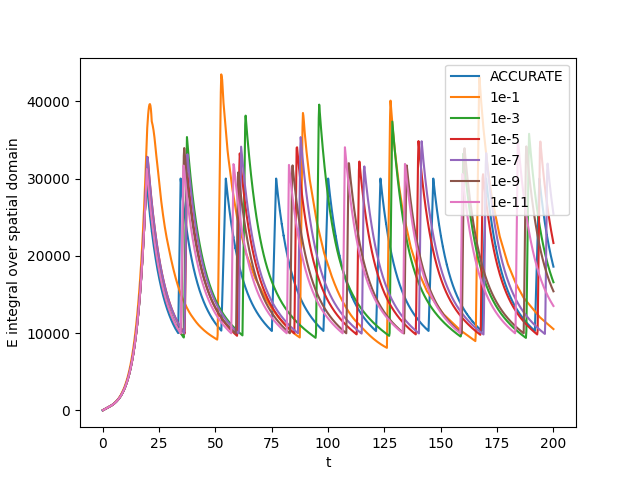
\includegraphics[width=0.7\linewidth]{./figures/pde_state_disc_tol_bacolikr_naive_1000}
\caption{Integral value plot of simple treatment of the state-dependent discontinuity problem at several tolerances using 1000 time intervals}
\label{fig:pde_state_disc_tol_bacolikr_naive_1000}
\end{figure}

\begin{figure}[H]
\centering
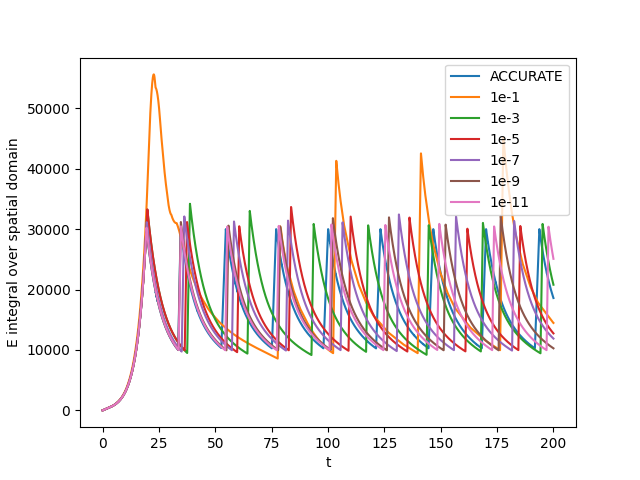
\includegraphics[width=0.7\linewidth]{./figures/pde_state_disc_tol_bacolikr_naive_10000}
\caption{Integral value plot of simple treatment of the state-dependent discontinuity problem at several tolerances using 10000 time intervals}
\label{fig:pde_state_disc_tol_bacolikr_naive_10000}
\end{figure}

Figures $\ref{fig:pde_state_disc_tol_bacolikr_naive_1000}$ and $\ref{fig:pde_state_disc_tol_bacolikr_naive_10000}$ show that the solutions at different tolerances with the simple implementation at 1000 and 10000 time intervals. We can see that increasing the number of time intervals does increase the accuracy of the solvers, as with 10000 steps, the solutions oscillate more cleanly between 10000 and 30000. We note that in both cases, very coarse tolerances like $10^{-1}$ and $10^{-3}$ provide very inaccurate solutions. Surprisingly, at very sharp tolerances like $10^{-9}$ and $10^{-11}$, the solutions are aligned with each other and with the more accurate solution up to the second root. However, even very sharp tolerances fail to provide accurate solutions for long-term forecasts. See Table $\ref{tab:pde_state_tol_study}$ and Table $\ref{tab:pde_state_tol_num_integrations}$ for an efficiency comparison between the simple implementation and the implementation that uses event detection. 

\paragraph{BACOLIKR with event detection}
\begin{figure}[H]
\centering
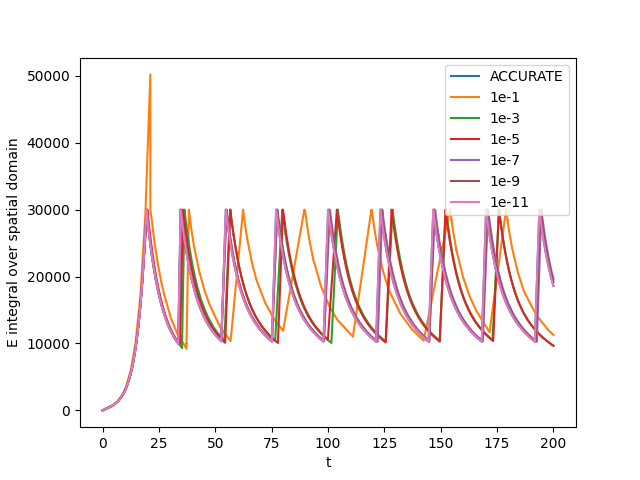
\includegraphics[width=0.7\linewidth]{./figures/pde_state_disc_tol_event}
\caption{Integral value plot of event detection solutions to state-dependent discontinuity problem at several tolerances}
\label{fig:pde_state_disc_tol_event}
\end{figure}

With event detection, the solutions oscillate correctly between 10000 and 30000 for all tolerances except for $10^{-1}$. The other solutions are only slightly misaligned but this can be explained because of the tolerance used in the root-finding function. Depending on the tolerance, the root is detected at a slightly different location by the root-finding algorithm and thus different tolerances lead to detection of the roots at slightly different times. These errors compound; the solutions are aligned for the first few roots but for accurate longer-term forecasts, a sharp tolerance is required. Despite this, event detection can provide accurate solutions at a tolerance of only $10^{-7}$, something which the simple implementation could not do even with 10000 time intervals at a tolerance of $10^{-11}$.

\paragraph{Efficiency of the solvers}
\begin{table}[h]
\caption {State-dependent discontinuity model tolerance study - number of function evaluations} 
\label{tab:pde_state_tol_study}
\begin{center}
\begin{tabular}{ c c c c } 
tolerance & simple 1000 & simple 10000 & with event detection \\ 
1e-1      &             101250   &              112600   &   137300 \\
1e-3      &             290600   &              343410   &   376855 \\
1e-5      &             848080   &              862960   &  1052920 \\
1e-7      &            2217610     &           2215690   &  3217450\\
1e-9      &            6040485     &           5811165   &  7915085  \\
1e-11     &           16402140     &          18508725   & 21256400 \\
\end{tabular}
\end{center}
\end{table}

\begin{table}[h]
\caption {Number of times the integration routine is called using event detection for the state-dependent discontinuity problem} 
\label{tab:pde_state_tol_num_integrations}
\begin{center}
\begin{tabular}{ c c } 
tolerance & number of calls to integration routine with event detection \\ 
1e-1      &    420 \\
1e-3      &    940 \\
1e-5      & 1634 \\
1e-7      & 3405 \\
1e-9      & 5059 \\
1e-11     & 9753 \\
\end{tabular}
\end{center}
\end{table}

Table $\ref{tab:pde_state_tol_study}$ shows that we are forced to sacrifice efficiency for accuracy in this problem. We note that all simple solutions depend highly on the time checking and thus should not be trusted for accurate solutions. Though they use fewer function evaluations than the event detection solutions of the same tolerance, the solutions they yield are not even reasonably accurate. 

We also note that Table $\ref{tab:pde_state_tol_num_integrations}$ shows that for the case of the simple implementation with 10000 time intervals, the integration routine is called less with event detection at all the tolerances as this simple implementation and all other implementations with more time intervals will call the integration routine more frequently (once at the end of each interval). The poor accuracy of the simple implementation of the solution to the state-dependent discontinuity problem should not be overlooked. Event detection is a better way of solving such problems with reasonable accuracy. 
%
%\end{document}
